\begin{figure}[H]
    \begin{subfigure}[t]{0.5\textwidth}
        \caption{}
        \centering
        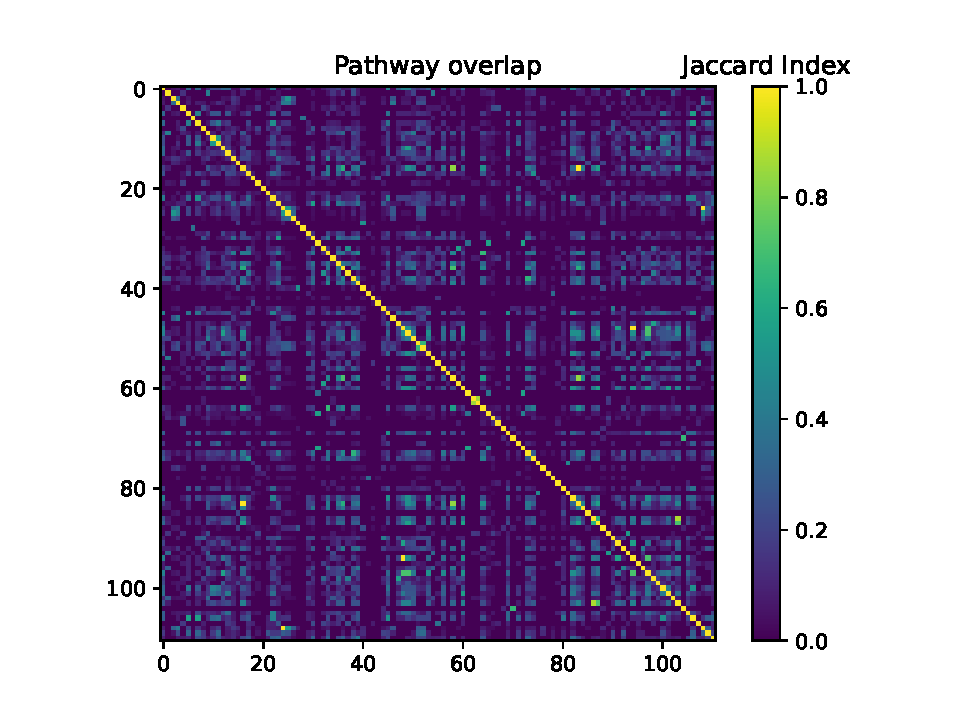
\includegraphics[width=0.8\textwidth]{/Users/djuna/Documents/ABCA7lof2/editorial_paper/main_panels_svgs/fs3/jaccard_mat_sub.pdf}        
    \end{subfigure}
    \begin{subfigure}[t]{0.5\textwidth}
        \caption{}
        \centering
        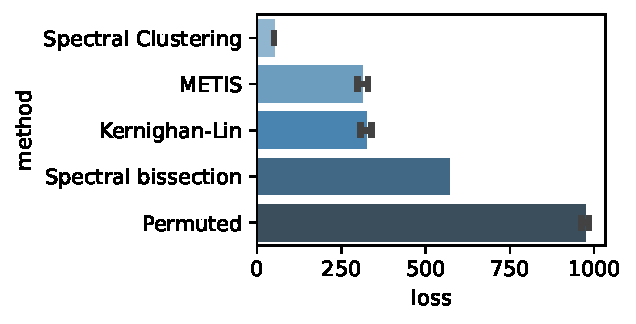
\includegraphics[width=0.8\textwidth]{/Users/djuna/Documents/ABCA7lof2/editorial_paper/main_panels_svgs/fs3/partitioning_losses.pdf}        
    \end{subfigure}
    \begin{subfigure}[t]{1\textwidth}
        \caption{}
        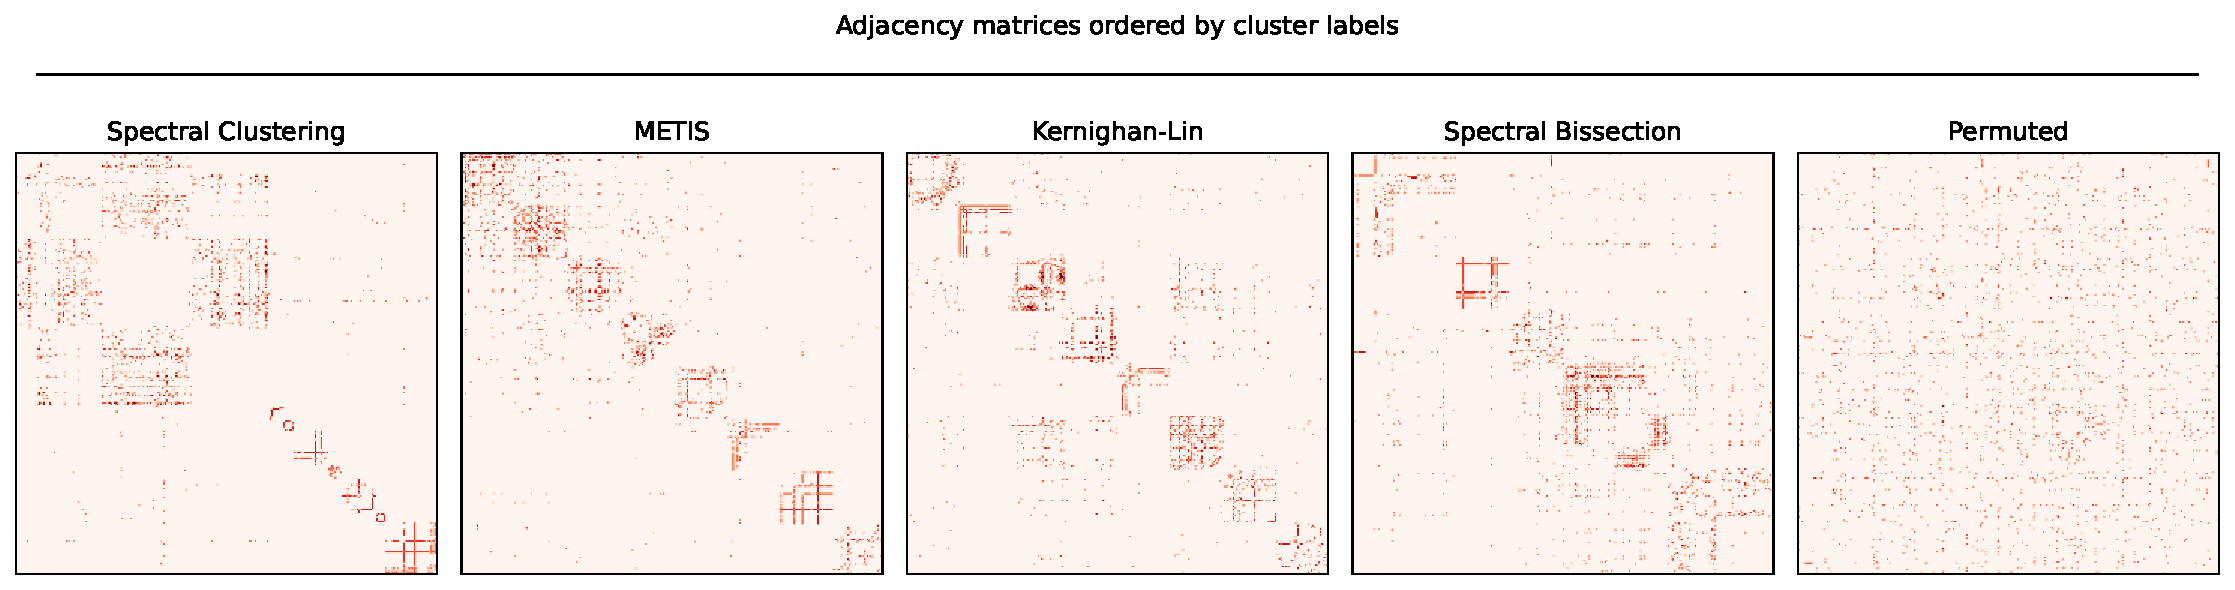
\includegraphics[width=\textwidth]{/Users/djuna/Documents/ABCA7lof2/editorial_paper/main_panels_svgs/fs3/adjacency_matrices_ordered_by_cluster_labels.pdf}        
    \end{subfigure}
    \begin{subfigure}[t]{0.33\textwidth}
        \caption{}
        \centering
        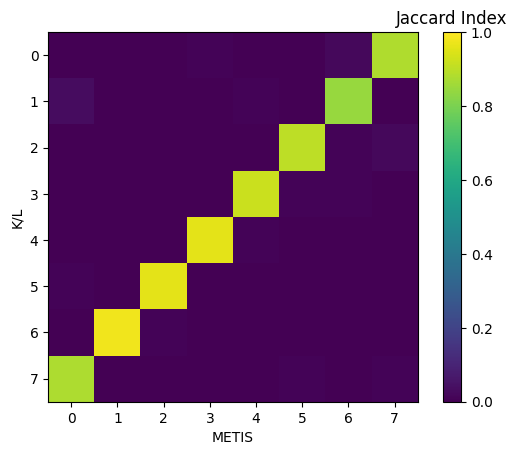
\includegraphics[width=0.8\textwidth]{/Users/djuna/Documents/ABCA7lof2/editorial_paper/main_panels_svgs/fs3/argmins_jaccard.pdf}        
    \end{subfigure}
    \begin{subfigure}[t]{0.33\textwidth}
        \caption{}
        \centering
        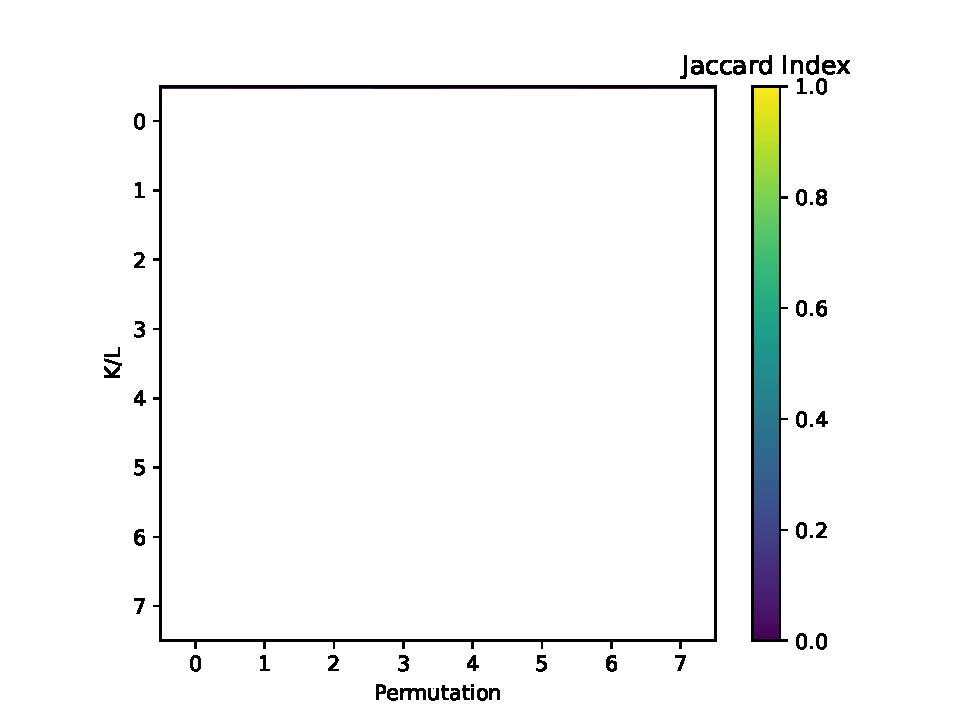
\includegraphics[width=0.8\textwidth]{/Users/djuna/Documents/ABCA7lof2/editorial_paper/main_panels_svgs/fs3/random_jaccard.pdf}        
    \end{subfigure}
    \begin{subfigure}[t]{0.33\textwidth}
        \caption{}
        \centering
        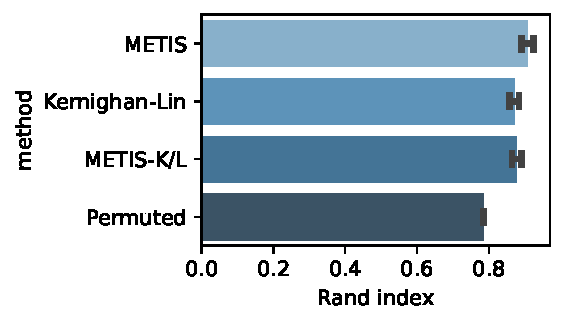
\includegraphics[width=0.8\textwidth]{/Users/djuna/Documents/ABCA7lof2/editorial_paper/main_panels_svgs/fs3/rand_indices.pdf}        
    \end{subfigure}
\end{figure}

\paragraph*{Fig. S3.} Benchmarking partitioning and clustering algorithms for gene–pathway grouping.

\phantomsection

\addcontentsline{toc}{paragraph}{Fig. S3.}

\textbf{a,} Analysis of Jaccard overlap between pathways conducted on an \( n \times p \) matrix, where the \( n \) pathways are a subset of the WikiPathways database that annotate more than four leading-edge (LE) genes as identified by fGSEA enrichment (unadjusted \( p<0.05 \)) comparing ABCA7 control versus LoF excitatory neurons (\( p \) total LE genes). \textbf{b,} Average loss (total cut size; Methods) from applying algorithms—spectral clustering (SC), METIS, Kernighan–Lin (K/L), spectral bisection (SB), and random permutation—to the graph \( G \) (\( n + p = 379 \) vertices; Methods). SC and random permutation were run over 1,000 initiations; METIS and K/L over \(5 \times 10^5\) initiations. SB is deterministic and was run once. Error bars indicate standard deviations. \textbf{c,} Unweighted adjacency matrix of graph \( G \), sorted by cluster labels assigned by each algorithm. Red indicates edges between vertices. Labels correspond to the best initiation (lowest loss) from 1,000 initiations (SC, random permutation) or \(5 \times 10^5\) initiations (METIS, K/L). \textbf{d,} Pairwise labeling consistency between optimal K/L and optimal METIS initiations. Axes represent cluster labels from each method; color intensity reflects the fraction of shared vertices per cluster. \textbf{e,} Same as (d) but comparing optimal K/L and optimal random permutation initiations. \textbf{f,} Average Rand index (RI) across initiation pairs from (b). “METIS,” “Kernighan–Lin,” and “Permuted” on the Y-axis indicate mean RI (label consistency) within each algorithm. “METIS–K/L” indicates mean RI for pairwise comparisons between METIS and K/L. Error bars show standard deviations. \( \text{RI} = \frac{\text{number of agreeing vertex pairs}}{\text{total vertex pairs}} \).

